\section{Технологический раздел}

\subsection{Архитектура приложения}

Для приложения была выбрана клиент-серверная архитектура. Доступ к серверной части будет осуществляться с помощью API~\cite{api}. Для осуществления запросов к базе данных будут использоваться коннекторы, предоставляющие интерфейс взаимодействия посредством языка программирования. Приложение было разделено на компоненты: компонент доступа к данным, компонент бизнес-логики, компонент интерфейса. Верхнеуровневое разбиение на компоненты представлено на рисунке~\ref{img:upper}.
\begin{figure}[!h]
	\centering
	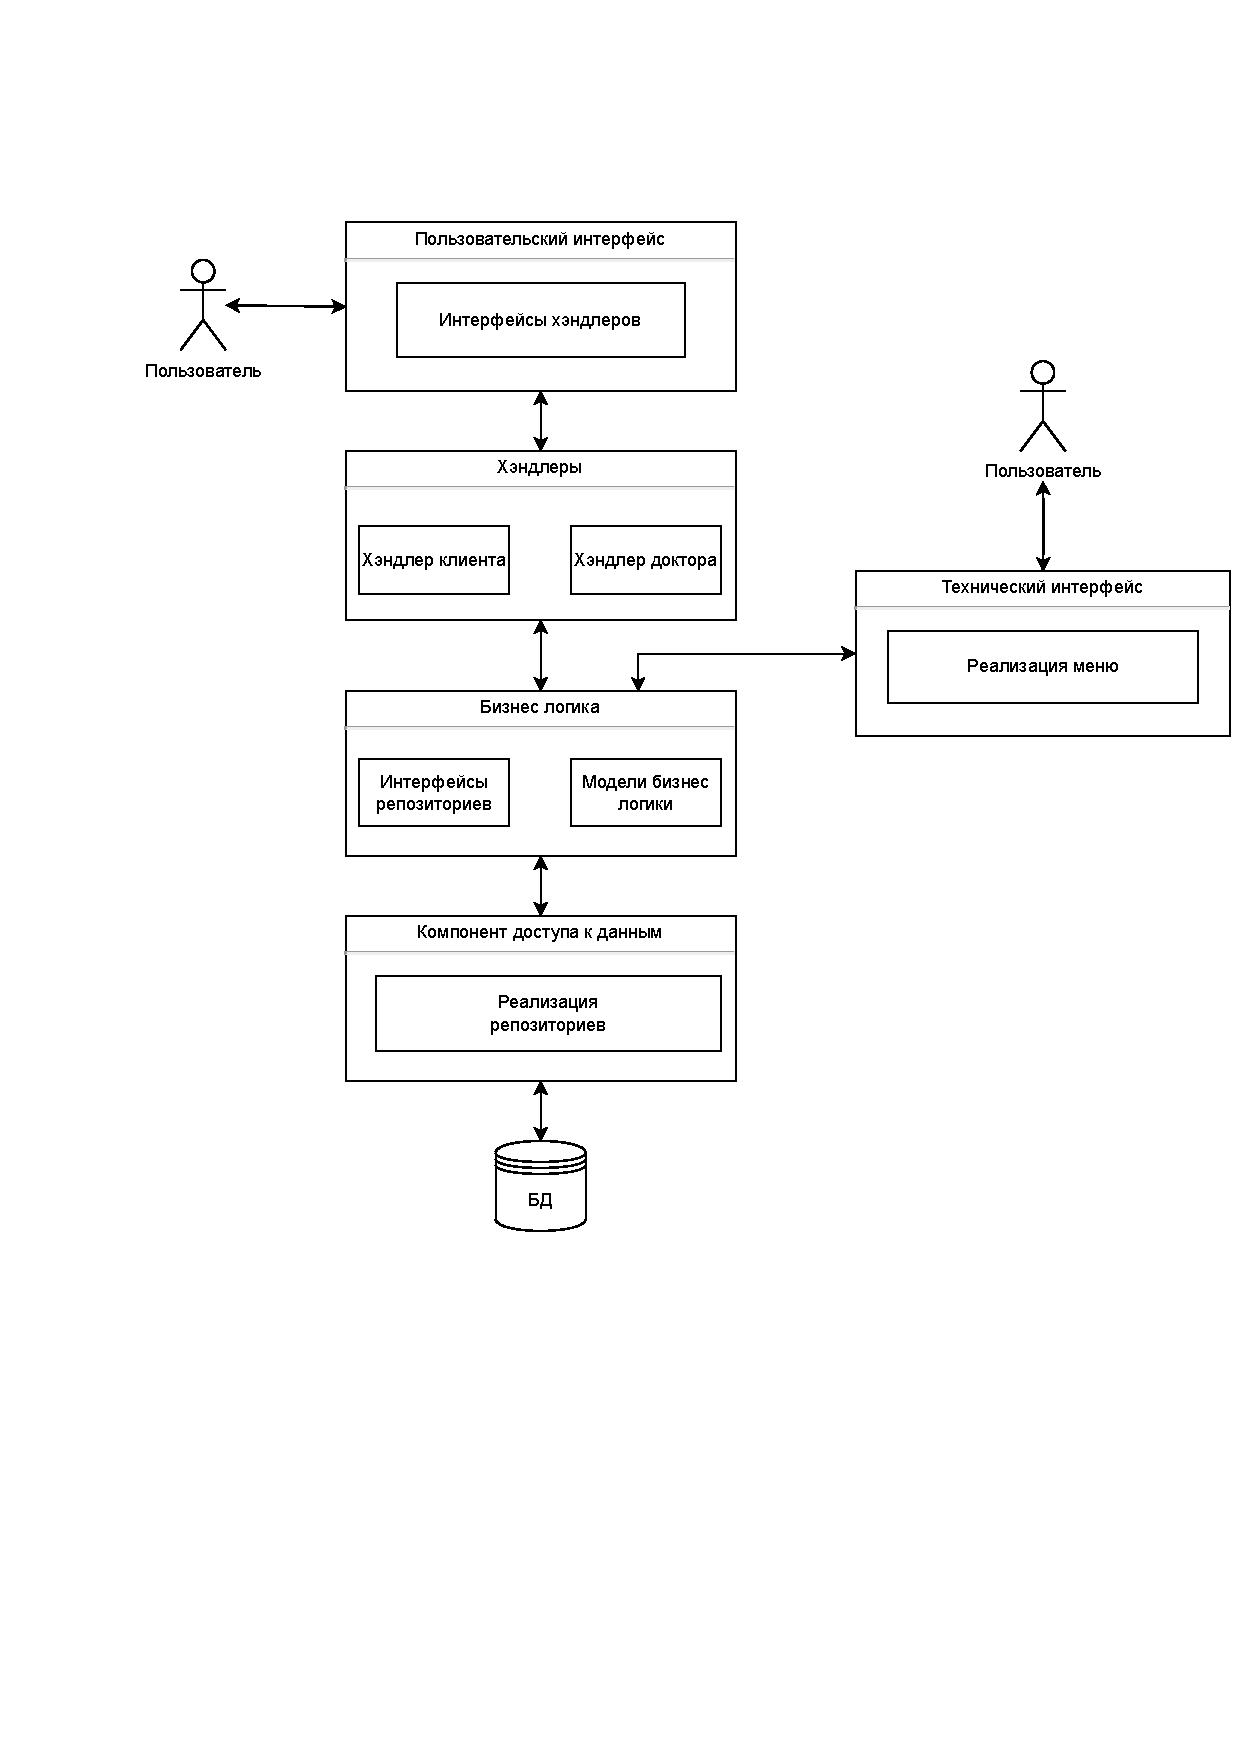
\includegraphics[width=165mm]{image/upper}
	\caption{Верхнеуровневое разбиение на компоненты}
	\label{img:upper}
\end{figure}

\newpage

\subsection{Средства реализации}

В рамках данной работы были выбраны следующие технологии.
\begin{enumerate}[label=\arabic*)]
	\item Язык программирования -- Golang~\cite{go}.
	\item Система управления базами данных -- PostgreSQL. 
	\item Для написания хранимых процедур базы данных будет использовано расширение языка SQL -- PL/pgSQL~\cite{pgSQL}.
	\item Для работы с СУБД была выбрана библиотека database/sql~\cite{go-sql}, предоставляющая универсальный интерфейс для реляционных баз данных, а также ее расширение -- библиотека sqlx~\cite{sqlx}.
	\item Фреймворк для реализации API -- gin~\cite{gin}.
	\item Для обечпечения безопасности паролей пользователей была использована хэш-функция bcrypt~\cite{bcrypt}. 
	\item Аутентификация была реализована на основе Bearer-токенов~\cite{bearer}.
	\item Для автоматизации развертывания и изолирования приложения была выбрана платформа Docker~\cite{docker}. 
	\item Технический интерфейс -- консоль. 
\end{enumerate}

\subsection{Детали реализации}

\subsubsection{Создание таблиц}

В листинге~\ref{tables} представлен код создания таблиц и ограничений, описанных ранее.

\begin{code} 
	\captionof{listing}{Скрипт создания таблиц}
	\label{tables}
	\inputminted
	[
	frame=single,
	framerule=0.5pt,
	framesep=10pt,
	fontsize=\small,
	tabsize=4,
	linenos,
	numbersep=5pt,
	xleftmargin=10pt,
	]
	{sql}
	{code/tables.sql}
\end{code}

\subsubsection{Создание ролей на уровне базы данных}

В конструкторской части были выделены 4 роли на уровне базы данных: гость, клиент, доктор и администратор. Создание ролей и выделение им прав, в соответствии с ролевой моделью, представлены в листинге~\ref{role}. 

\begin{code} 
	\captionof{listing}{Скрипт создания ролевой модели базы данных}
	\label{role}
	\inputminted
	[
	frame=single,
	framerule=0.5pt,
	framesep=10pt,
	fontsize=\small,
	tabsize=4,
	linenos,
	numbersep=5pt,
	xleftmargin=10pt,
	]
	{sql}
	{code/roles.sql}
\end{code}

\subsubsection{Создание триггера}

В конструкторской части был разработан триггер для проверки валидности новой записи с помощью расширения PL/pgSQL, используемого в СУБД PostgreSQL. Код триггера представлен в листинге~\ref{func}. 

\begin{code} 
	\captionof{listing}{Триггер проверки валидности новой записи}
	\label{func}
	\inputminted
	[
	frame=single,
	framerule=0.5pt,
	framesep=10pt,
	fontsize=\small,
	tabsize=4,
	linenos,
	numbersep=5pt,
	xleftmargin=10pt,
	]
	{sql}
	{code/func.sql}
\end{code}

\subsection{Тестирование}

Для тестирования проекта были реализованы модульные тесты для компонента доступа к данным и для компонента бизнес-логики. Также написаны интеграционные тесты для связи двух компонентов. Каждый тест выполняется в отдельном Docker контейнере, до теста запускается скрипт создания таблиц и в случае необходимости база данных заполняется тестовыми данными. 

Для автоматизации тестирования, проведения исследования и развертывания использовался инструмент Gitlab CI/CD~\cite{ci}. Был создан сценарий, состоящий из четырех стадий. 
\begin{enumerate}[label=\arabic*)]
	\item Pre. Стадия состоит из статического анализа кода и инициализации модулей. 
	\item Test. Стадия содержит модульное тестирование компонента бизнес-логики и компонента доступа к данным, а также интеграционное тестирования.
	\item Build. Состоит из сборки серверной части приложения и технического интерфейса.
	\item Research. Содержит исследование, описанное в следующем разделе.
\end{enumerate}
Задания, входящие в каждую из стадий приведены на рисунке~\ref{stages}. 
\begin{figure}[!h]
	\centering
	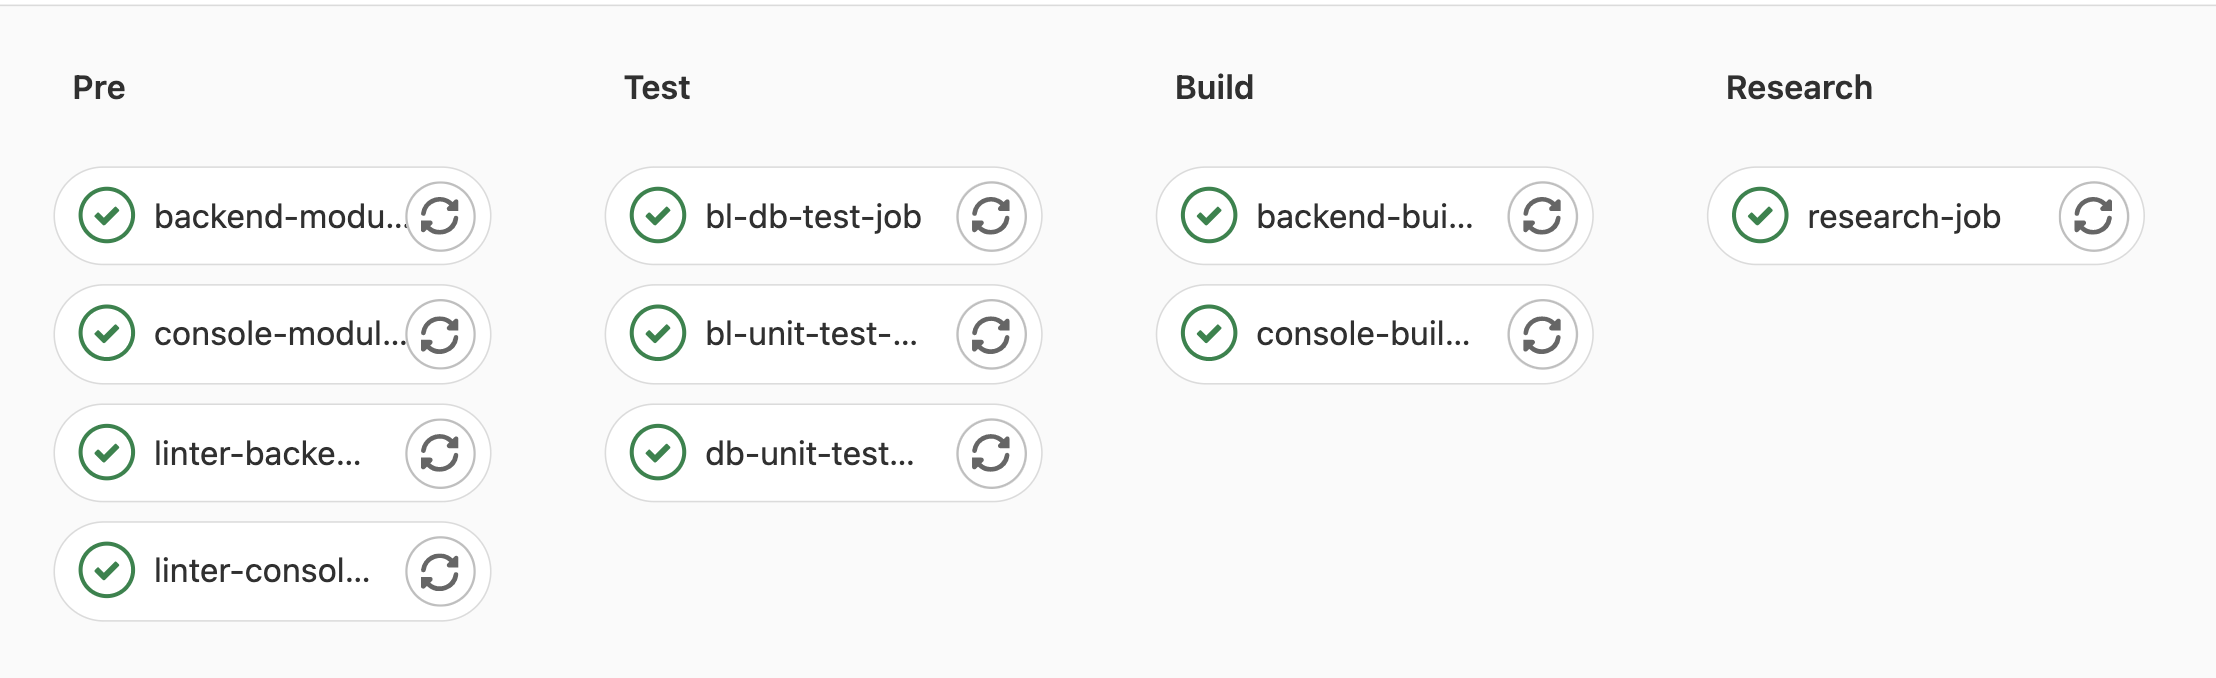
\includegraphics[width=\textwidth]{image/stages}
	\caption{Стадии сборочной линии}
	\label{stages}
\end{figure}

Серверная часть приложения и технический интерфейс не связаны между собой, но имеют общие стадии. На рисунке~\ref{needs} изображена зависимости между заданиями сборочной линии. 
\begin{figure}[!h]
	\centering
	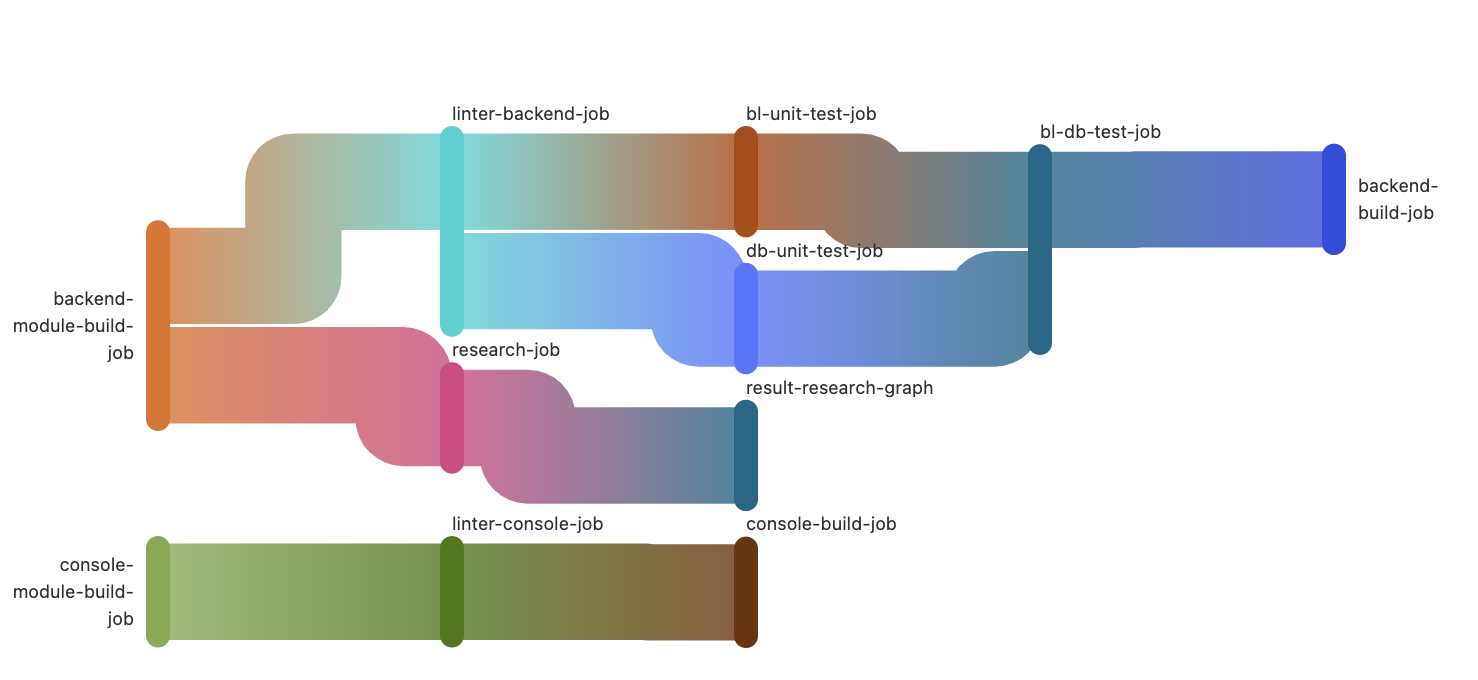
\includegraphics[width=\textwidth]{image/needs}
	\caption{Зависимости между заданиями}
	\label{needs}
\end{figure}

\subsection*{Вывод}
В данном разделе была описана архитектура приложения, средства и детали его реализации. Приведена сборочная линии для тестирования и развертывания приложения, а также проведения исследования с помощью инструмента Gitlab CI/CD.

